\begin{figure}[h!]
   \centering
   \begin{subfigure}[b]{0.4\textwidth}
      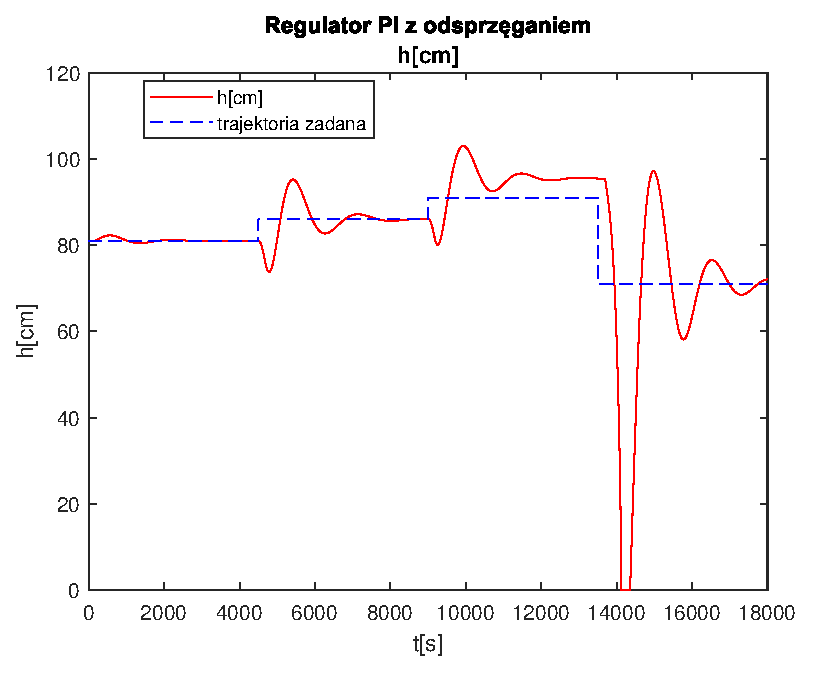
\includegraphics[width=1\linewidth]{img/PI/decoupler/noDisturbance/PIDecouplerH1Lintrue.eps}
      \caption{}
      \label{fig:fig:PIDecoupler1Lintrue1}
   \end{subfigure}
       
   \begin{subfigure}[b]{0.4\textwidth}
      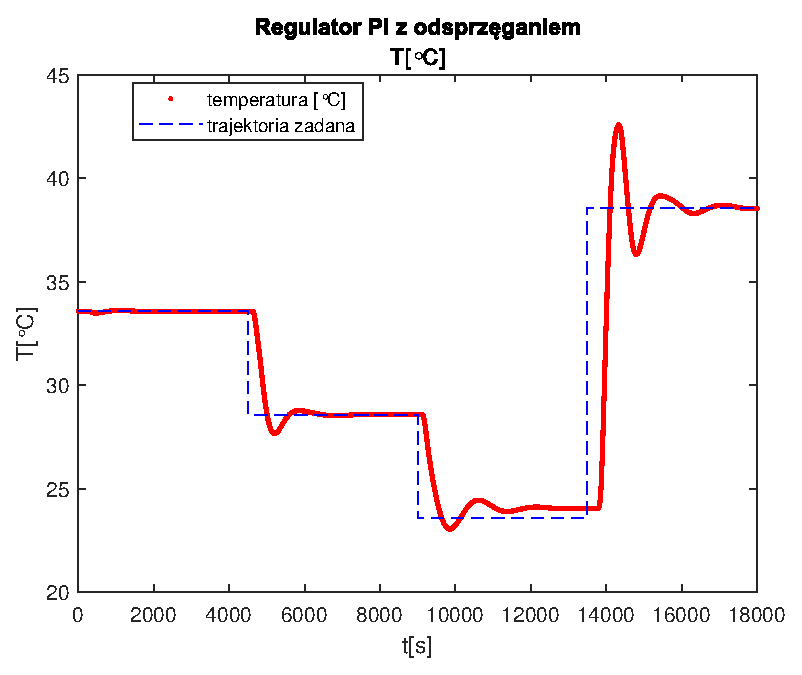
\includegraphics[width=1\linewidth]{img/PI/decoupler/noDisturbance/PIDecouplerT1Lintrue.eps}
      \caption{}
      \label{fig:fig:PIDecoupler1Lintrue2}
   \end{subfigure}
       
   \begin{subfigure}[b]{0.4\textwidth}
      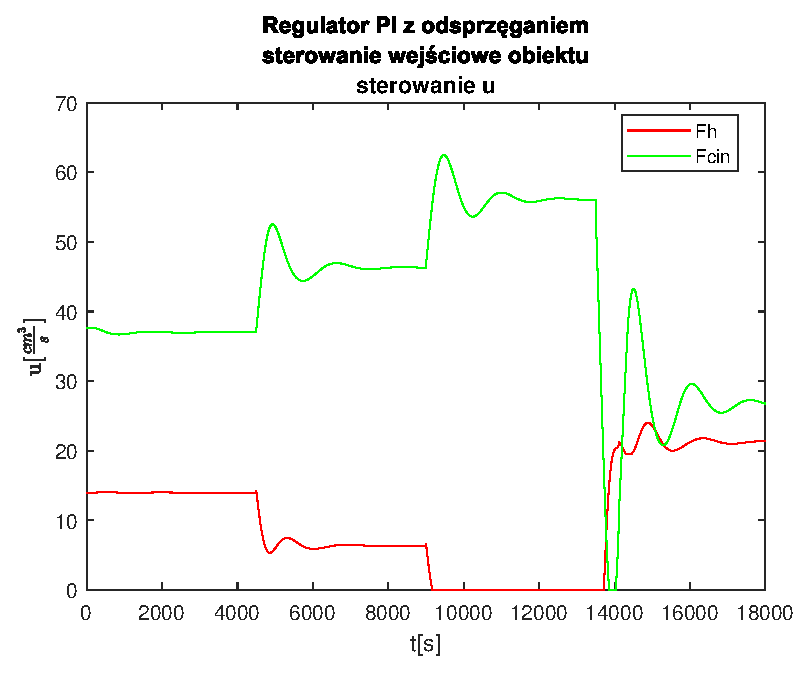
\includegraphics[width=1\linewidth]{img/PI/decoupler/noDisturbance/PIDecouplerControl1Lintrue.eps}
      \caption{}
      \label{fig:fig:PIDecoupler1Lintrue3}
   \end{subfigure}
    
   \begin{subfigure}[b]{0.4\textwidth}
      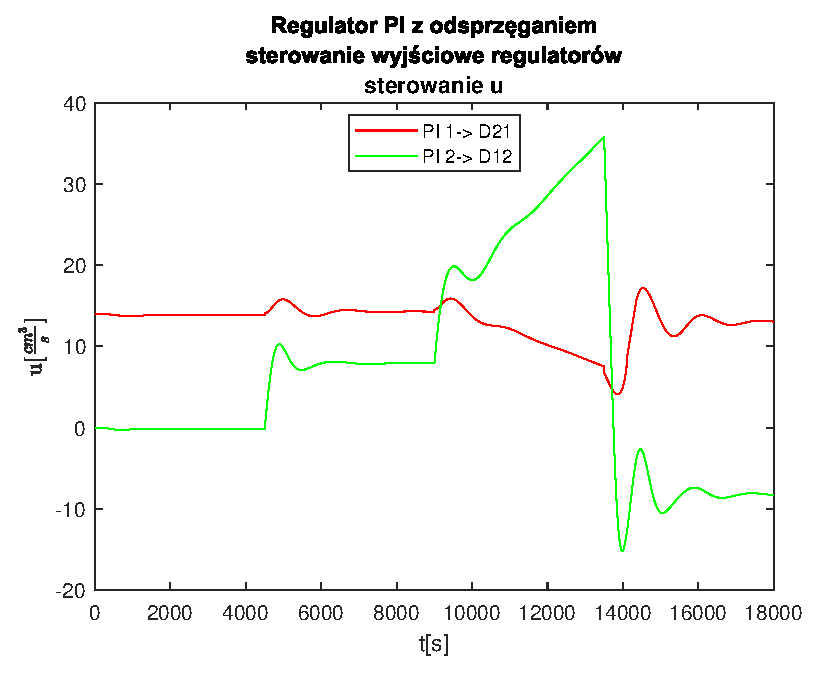
\includegraphics[width=1\linewidth]{img/PI/decoupler/noDisturbance/PIDecouplerControlD1Lintrue.eps}
      \caption{}
      \label{fig:fig:PIDecoupler1Lintrue4}
   \end{subfigure}
       
   \caption{Wykresy dla regulatora PI z odsprzeganiem.}
   \label{fig:PIDecoupler1Lintrue}
\end{figure}
           
\begin{figure}[h!]
   \centering
   \begin{subfigure}[b]{0.4\textwidth}
      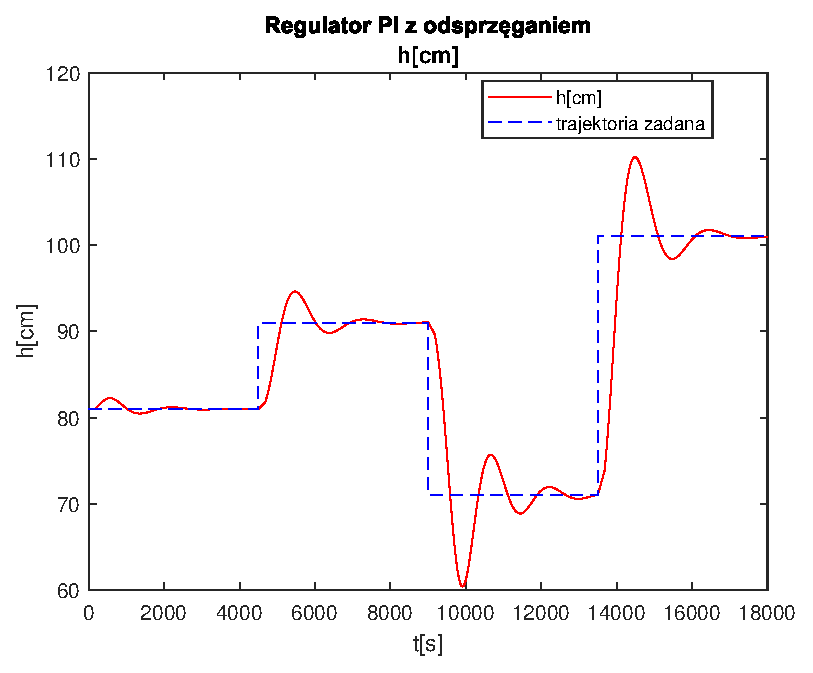
\includegraphics[width=1\linewidth]{img/PI/decoupler/noDisturbance/PIDecouplerH2Lintrue.eps}
      \caption{}
      \label{fig:fig:PIDecoupler2Lintrue1}
   \end{subfigure}
       
   \begin{subfigure}[b]{0.4\textwidth}
      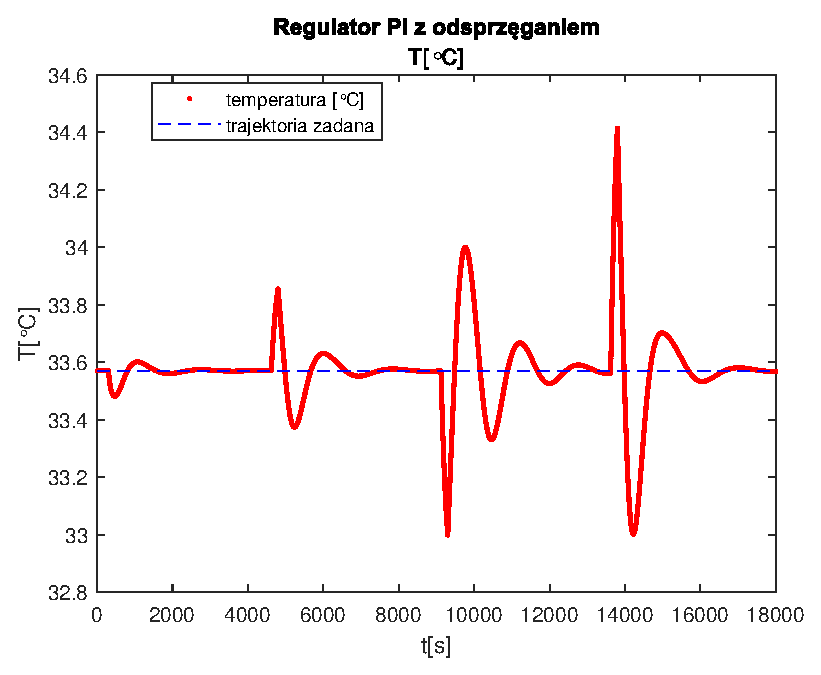
\includegraphics[width=1\linewidth]{img/PI/decoupler/noDisturbance/PIDecouplerT2Lintrue.eps}
      \caption{}
      \label{fig:fig:PIDecoupler2Lintrue2}
   \end{subfigure}
       
   \begin{subfigure}[b]{0.4\textwidth}
      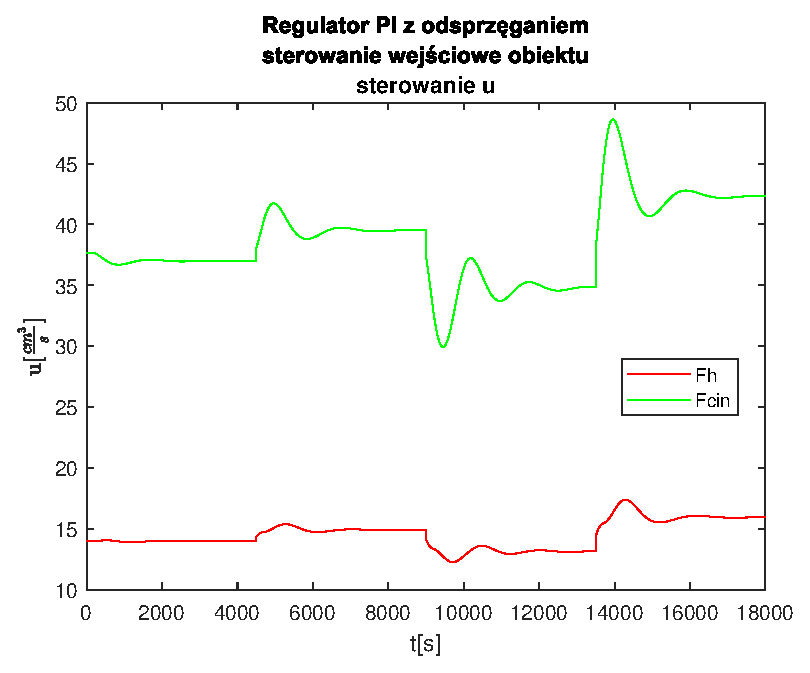
\includegraphics[width=1\linewidth]{img/PI/decoupler/noDisturbance/PIDecouplerControl2Lintrue.eps}
      \caption{}
      \label{fig:fig:PIDecoupler2Lintrue3}
   \end{subfigure}
       
   \begin{subfigure}[b]{0.4\textwidth}
      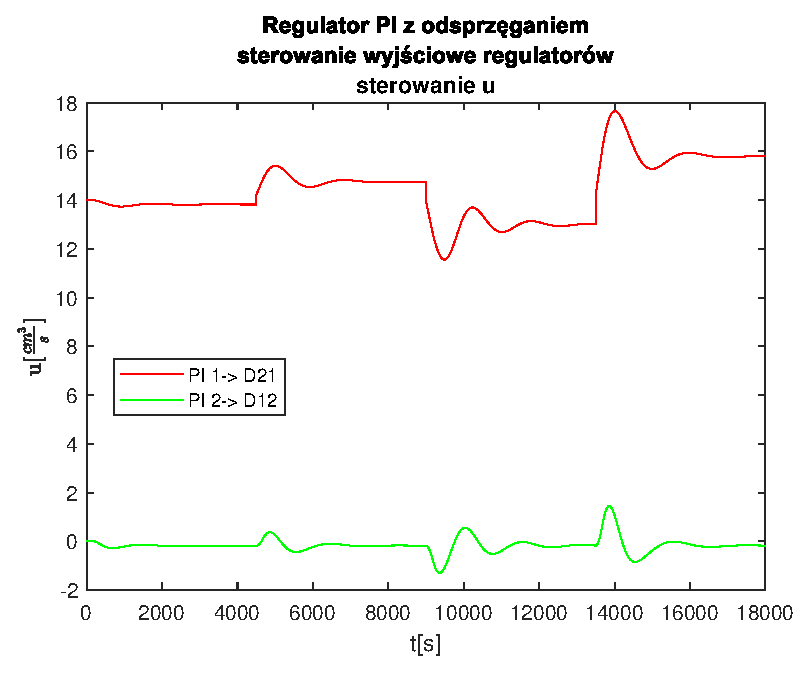
\includegraphics[width=1\linewidth]{img/PI/decoupler/noDisturbance/PIDecouplerControlD2Lintrue.eps}
      \caption{}
      \label{fig:fig:PIDecoupler2Lintrue4}
   \end{subfigure}
       
   \caption{Wykresy dla regulatora PI z odsprzeganiem.}
   \label{fig:PIDecoupler2Lintrue}
\end{figure}
           
\begin{figure}[h!]
   \centering
   \begin{subfigure}[b]{0.4\textwidth}
      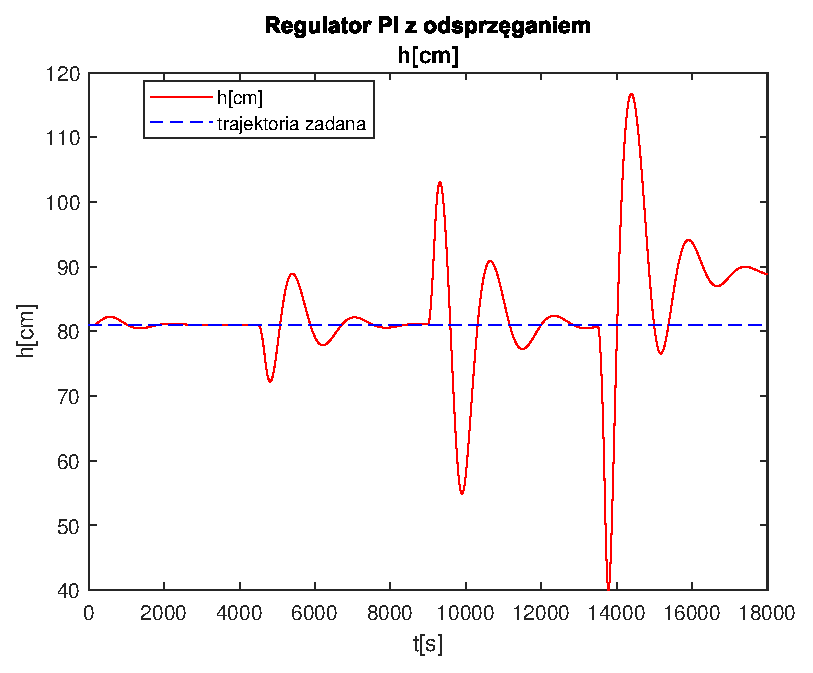
\includegraphics[width=1\linewidth]{img/PI/decoupler/noDisturbance/PIDecouplerH3Lintrue.eps}
      \caption{}
      \label{fig:fig:PIDecoupler3Lintrue1}
   \end{subfigure}
       
   \begin{subfigure}[b]{0.4\textwidth}
      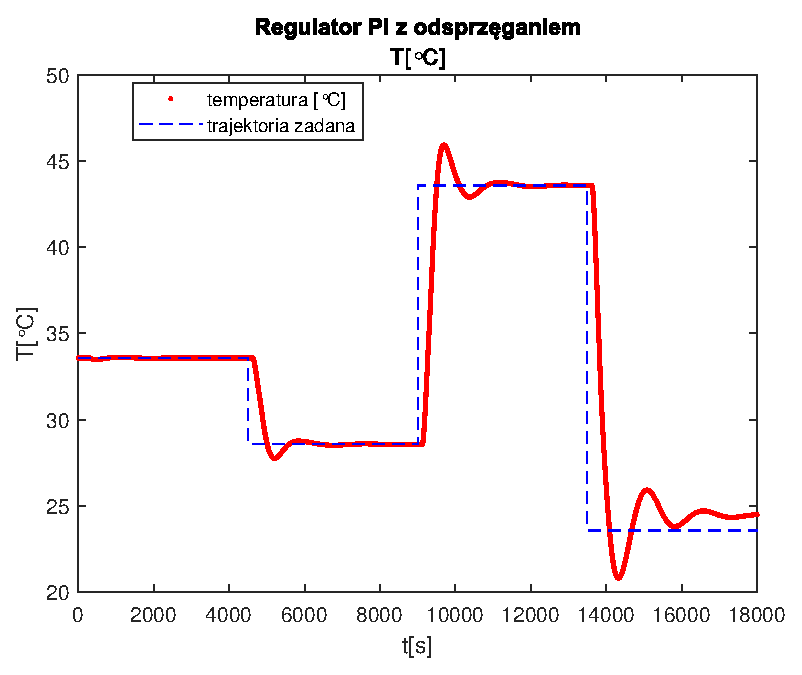
\includegraphics[width=1\linewidth]{img/PI/decoupler/noDisturbance/PIDecouplerT3Lintrue.eps}
      \caption{}
      \label{fig:fig:PIDecoupler3Lintrue2}
   \end{subfigure}
       
   \begin{subfigure}[b]{0.4\textwidth}
      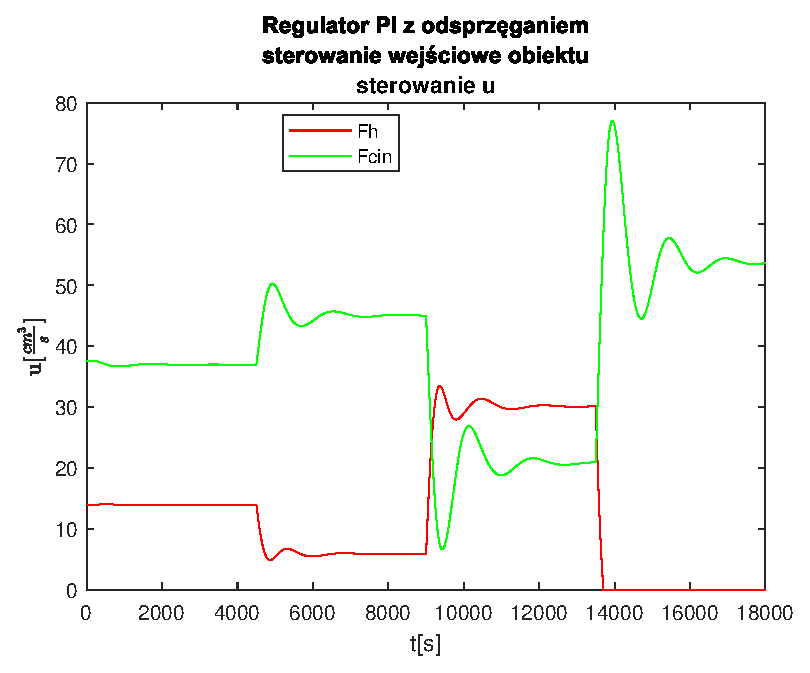
\includegraphics[width=1\linewidth]{img/PI/decoupler/noDisturbance/PIDecouplerControl3Lintrue.eps}
      \caption{}
      \label{fig:fig:PIDecoupler3Lintrue3}
   \end{subfigure}
       
   \begin{subfigure}[b]{0.4\textwidth}
      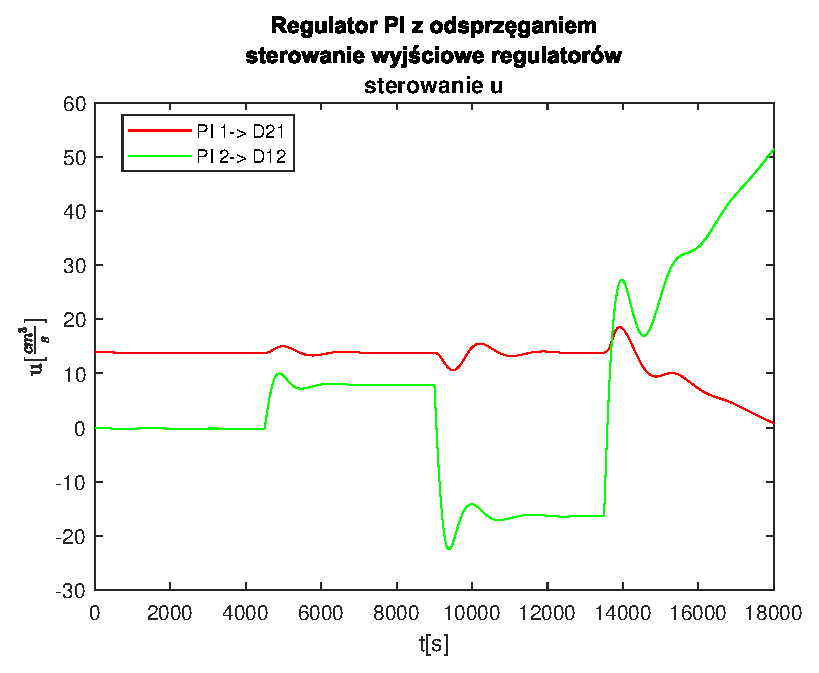
\includegraphics[width=1\linewidth]{img/PI/decoupler/noDisturbance/PIDecouplerControlD3Lintrue.eps}
      \caption{}
      \label{fig:fig:PIDecoupler3Lintrue4}
   \end{subfigure}
       
   \caption{Wykresy dla regulatora PI z odsprzeganiem.}
   \label{fig:PIDecoupler3Lintrue}
\end{figure}
           
